\documentclass[final]{beamer}

\usepackage[scale=1.24]{beamerposter}
\usetheme{confposter}
\setbeamercolor{block title}{fg=ngreen,bg=white}
\setbeamercolor{block body}{fg=black,bg=white}
\setbeamercolor{block alerted title}{fg=white,bg=dblue!70}
\setbeamercolor{block alerted body}{fg=black,bg=dblue!10}

\newlength{\sepwid}
\newlength{\onecolwid}
\newlength{\twocolwid}
\newlength{\threecolwid}
\setlength{\paperwidth}{48in} % A0 width: 46.8in
\setlength{\paperheight}{34in} % A0 height: 33.1in
\setlength{\sepwid}{0.024\paperwidth} % Separation width (white space) between columns
\setlength{\onecolwid}{0.22\paperwidth} % Width of one column
\setlength{\twocolwid}{0.464\paperwidth} % Width of two columns
\setlength{\threecolwid}{0.708\paperwidth} % Width of three columns
\setlength{\topmargin}{-0.5in} % Reduce the top margin size
%-----------------------------------------------------------

\usepackage{graphicx}  % Required for including images

\usepackage{booktabs} % Top and bottom rules for tables

\usepackage{hyperref}
\hypersetup{
    colorlinks=true,
    linkcolor=blue,
    filecolor=magenta,      
    urlcolor=blue,
}

\usepackage{amsmath}

\title{Close Encounter: 3122 Florence (1981 ET3) } % Poster title

\author{Bosscha Observatory $\vert$ Astronomy Research Division, ITB}

\institute{This information is generated on 2017-09-07 16:57 UTC.} 

\begin{document}

\addtobeamertemplate{block end}{}{\vspace*{2ex}}
\addtobeamertemplate{block alerted end}{}{\vspace*{2ex}}

\setlength{\belowcaptionskip}{2ex}
\setlength\belowdisplayshortskip{2ex}

\begin{frame}[t]

\begin{columns}[t] 

% First Column

\begin{column}{\sepwid}\end{column}

\begin{column}{\onecolwid}

\begin{alertblock}{Basic Properties}
\begin{itemize}
\item Name: 3122 Florence (1981 ET3)\item Discovered 1981-Mar-02 by Bus, S. J. at Siding Spring 
\item Estimated diameter: 4.02 \--- 8.99 km
\item Classification: Amor (NEO, PHA)
\item H: 14.1
\item Period: 859.486 days
\end{itemize}
\begin{table}
\caption{Orbital elements at epoch 2458000.5 JD }
\begin{tabular}{l c r}
\toprule
\textbf{Parameter} & & \textbf{    Value    } \\
\midrule Semi-major axis ($a$) & & 1.76913 \\ 
Eccentricity ($e$) & & .423300 \\ 
Inclination ($i$) & & 22.1507 \\ 
Lon. of ascending node ($\Omega$) & & 336.095 \\ 
Argument of pericenter ($\omega$) & & 27.8469 \\ 
Mean Anomaly ($M$) & & 351.438 \\ 
\bottomrule
\end{tabular}
\end{table}

\end{alertblock}


\begin{block}{Orbit}
\begin{figure}
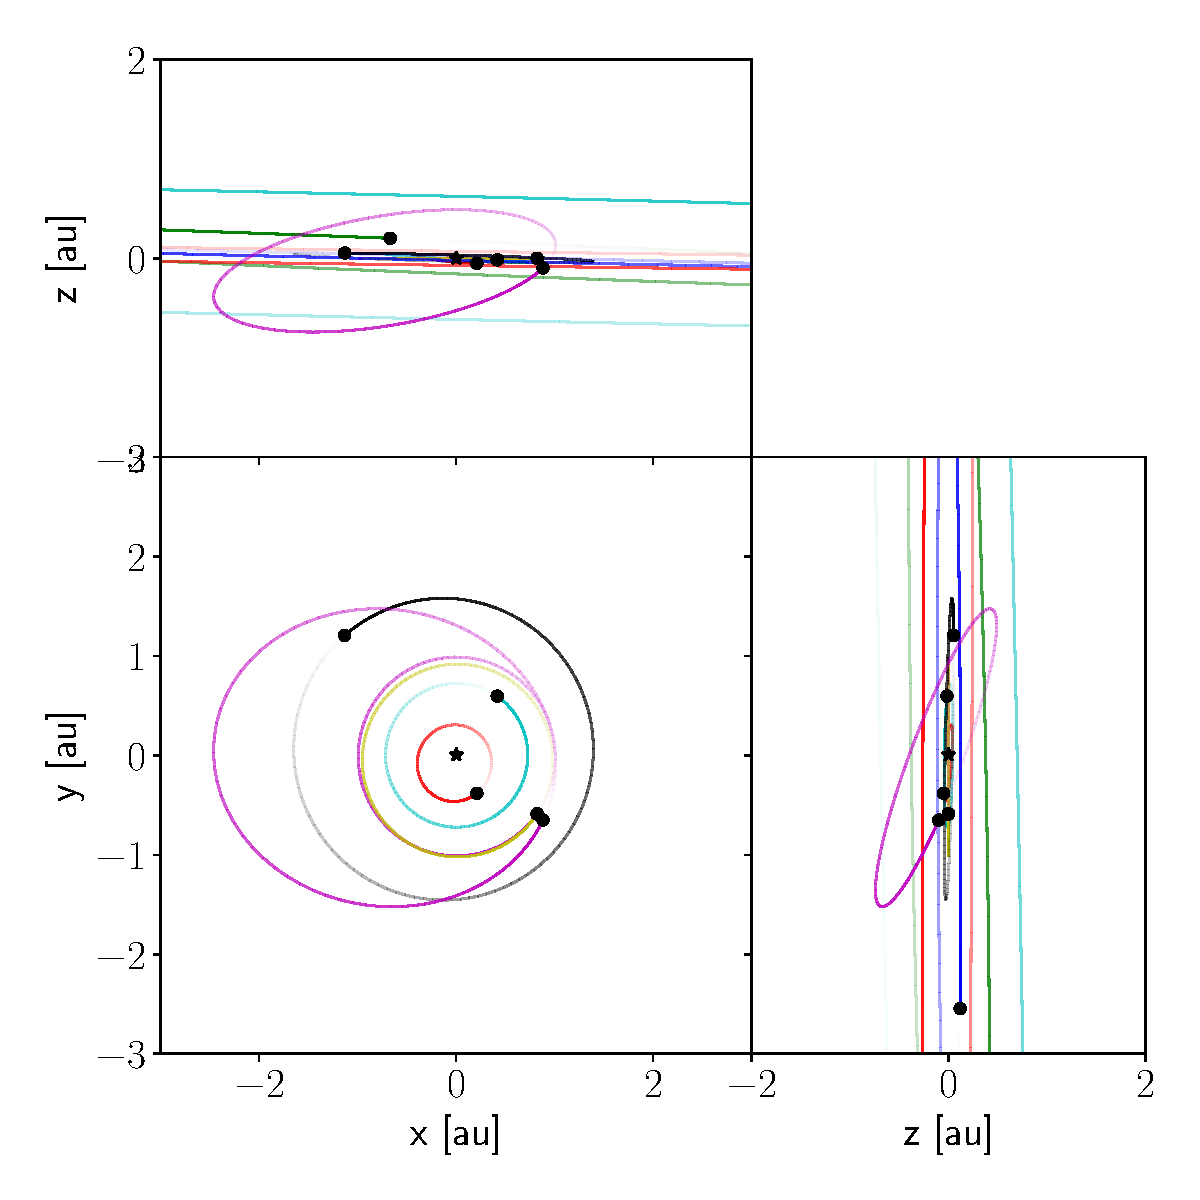
\includegraphics[width=0.99\textwidth]{initial_orbit.pdf}
\caption{Orbit of the asteroid and the planets. This plot only shows the inner region of the Solar System.}
\end{figure}
\end{block}

\begin{alertblock}{Acknowledgements}
Our script retrieve basic informations and initial condition from \href{https://ssd.jpl.nasa.gov/}{JPL NASA}, re-integrate the Solar System using \href{https://github.com/hannorein/rebound}{\texttt{Rebound}} package, and write this report using \LaTeX.
\end{alertblock}

\end{column}

% Second column

\begin{column}{\sepwid}\end{column}

\begin{column}{\twocolwid}

\begin{block}{Distance to the Earth and Orbital Elements}
\begin{figure}
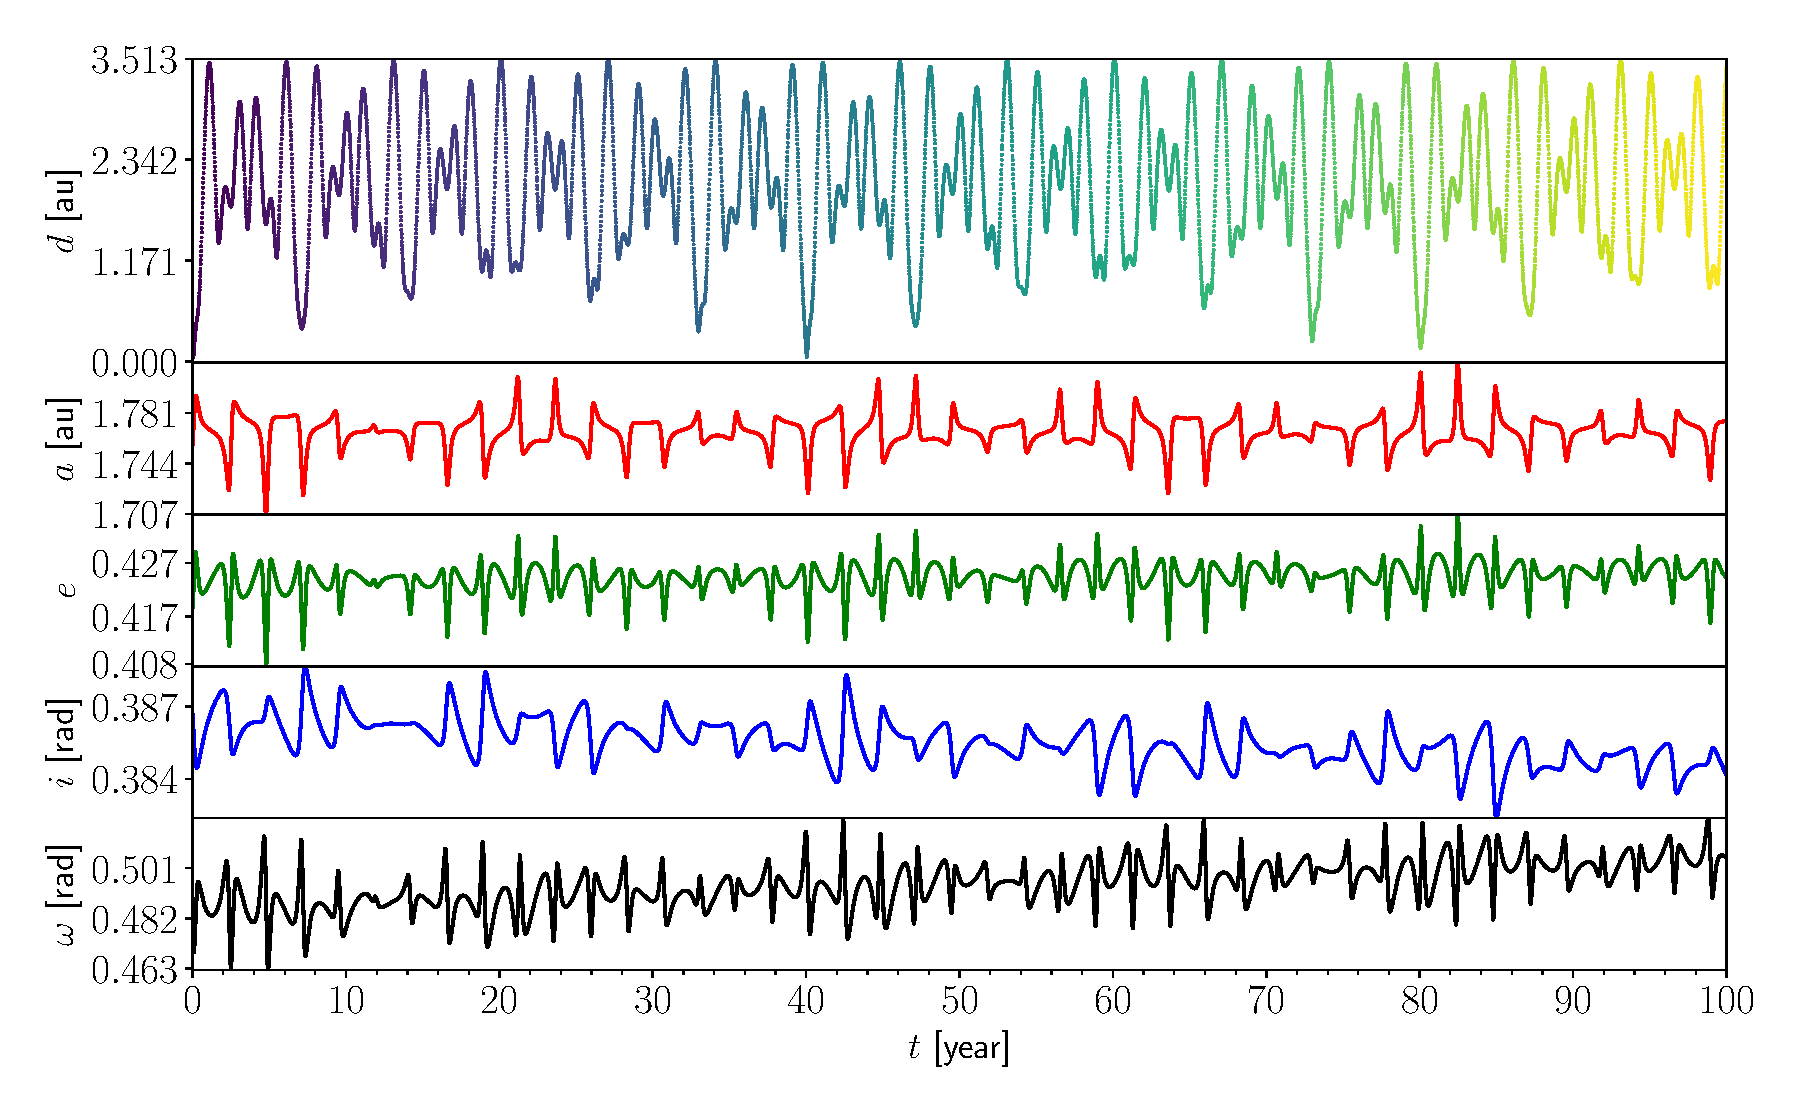
\includegraphics[width=0.99\linewidth]{daeiw.pdf}
\caption{Distance to the Earth and orbital elements of the asteroid for the next 100 years. Starting time of the integration is 2017-08-17 00:00 UTC.}
\end{figure}
\end{block}

\begin{columns}[t, totalwidth=\twocolwid] % Split up the two columns wide column

\begin{column}{\onecolwid}\vspace{-.6in}
\begin{block}{Geocentric}
\begin{figure}
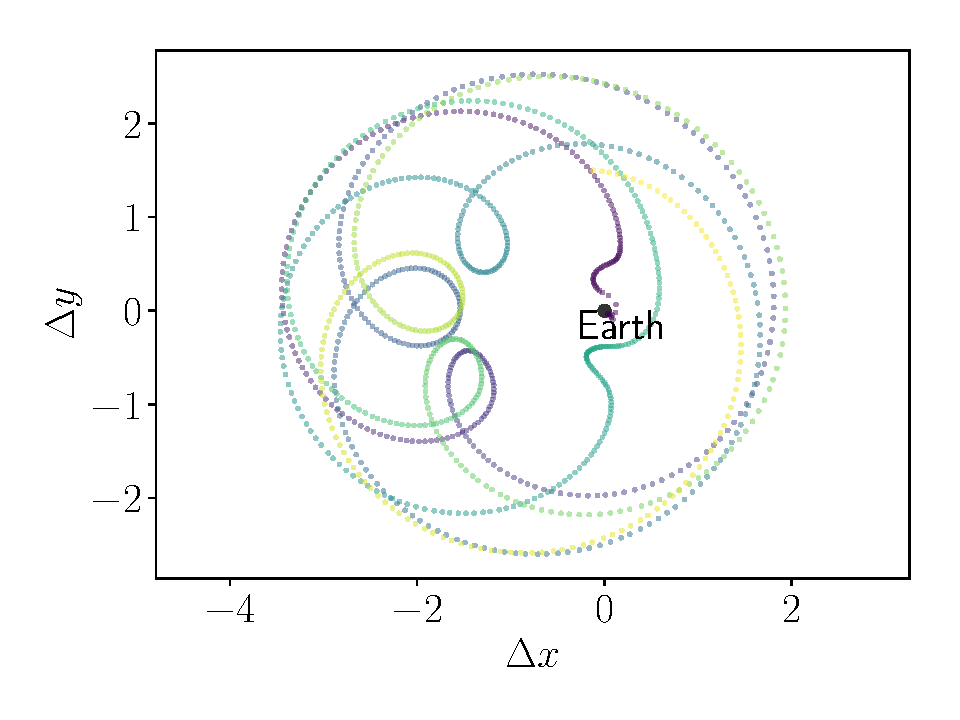
\includegraphics[width=0.99\textwidth]{geocentric.pdf}
\caption{Movement of the asteroid relative to the Earth ($xy$-plane; only the first 12 years of integration).}
\end{figure}
\end{block}
\end{column}

\begin{column}{\onecolwid}\vspace{-.6in} 
\begin{block}{Rotating Frame}
\begin{figure}
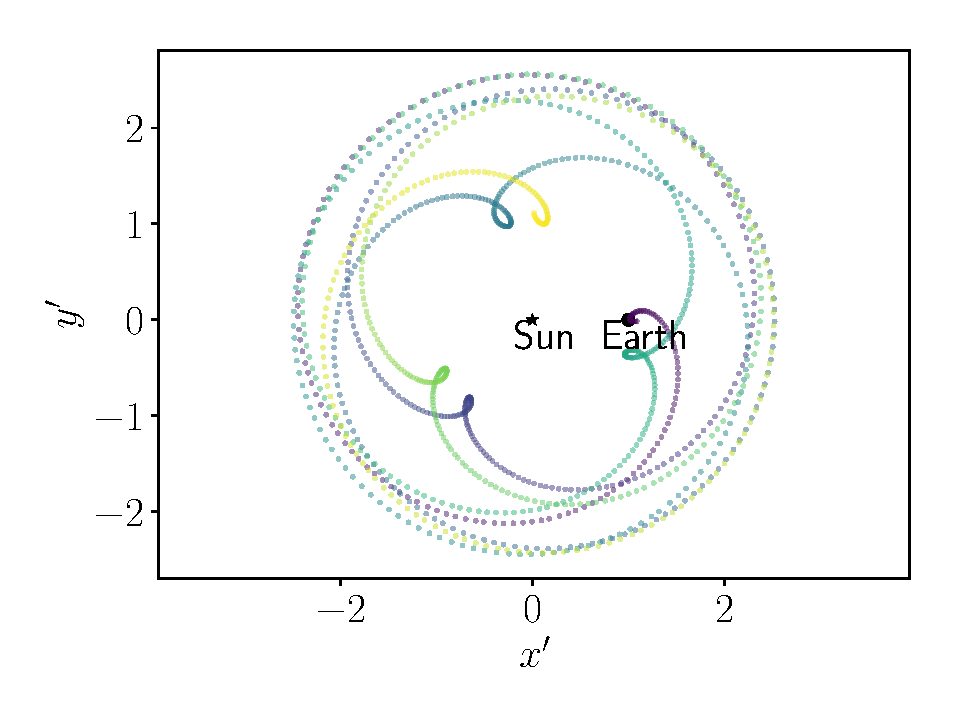
\includegraphics[width=0.99\textwidth]{rotframe.pdf}
\caption{Movement of the asteroid relative to the Sun-Earth system ($xy$-plane; only the first 12 years of integration).}
\end{figure}
\end{block}
\end{column}

\end{columns} 

\end{column} 


%%%% 
\begin{column}{\sepwid}\end{column} 

\begin{column}{\onecolwid} 

\setbeamercolor{block alerted title}{fg=black,bg=norange}
\setbeamercolor{block alerted body}{fg=black,bg=norange!10}

\begin{alertblock}{Nearest close encounter}
\begin{itemize}
\item Time: 1 September 2017, 12.05 UT
\item Distance:  $ 7.066 \times 10^6$ km ($18.38$ Lunar Distance)
\item Relative velocity: 
\end{itemize}
\end{alertblock}


\begin{alertblock}{List of close encounter}
\begin{table}
\vspace{2ex}
\begin{tabular}{l c c c}
\toprule
\textbf{Time} & \textbf{   Body   } & \textbf{  $\boldsymbol{d}$ (au)  } & \textbf{$\boldsymbol{v_{rel}}$ (km/s)} \\
\midrule2017-09-01 & Earth & 0.0472 & 13.53 \\ 
2024-10-01 & Earth & 0.3816 & 15.30 \\ 
2050-08-11 & Earth & 0.3481 & 19.51 \\ 
2057-09-02 & Earth & 0.0499 & 13.47 \\ 
2064-10-05 & Earth & 0.4166 & 15.95 \\ 
2090-08-17 & Earth & 0.2340 & 17.16 \\ 
2097-09-11 & Earth & 0.1558 & 12.99 \\ 
2123-08-05 & Earth & 0.4723 & 22.49 \\ 
2130-08-27 & Earth & 0.0869 & 14.60 \\ 
2137-09-24 & Earth & 0.2891 & 13.81 \\ 
2163-08-07 & Earth & 0.4379 & 21.70 \\ 
2170-08-28 & Earth & 0.0781 & 14.49 \\ 
2177-09-22 & Earth & 0.2720 & 13.59 \\ 
\bottomrule
\end{tabular}
%\caption{Word Formation}
\end{table}
\end{alertblock}

\end{column} 


\end{columns} 
\end{frame}
\end{document}